\icode{O-EMA-SU-261001}
\begin{figure}[htbp]
		\centering
		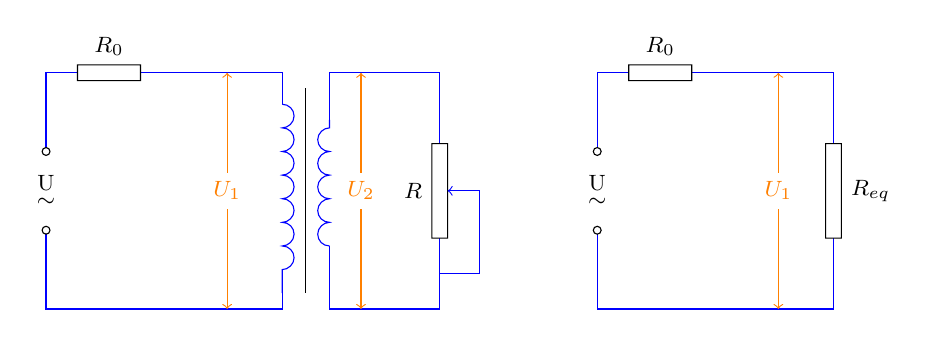
\begin{tikzpicture}[decoration={bumps,segment length=6mm,amplitude=1.5mm}]
			\draw[blue] (0,2)--(0,3)--(3,3)--(3,2.6) (0,1)--(0,0)--(3,0)--(3,.4);
			\draw[decorate,blue] (3,2.6)--(3,.2);
			\draw[blue,decorate] (3.6,.8)--(3.6,2.4);
			\draw[blue] (3.6,2.4)--(3.6,3)--(5,3)--(5,0)--(3.6,0)--(3.6,.8);
			\draw (3.3,2.8)--(3.3,.2);
			\filldraw[fill=white] (0,1) circle(.05) (0,2) circle(.05) (.4,2.9) rectangle(1.2,3.1) (4.9,.9) rectangle(5.1,2.1);
			\draw[blue,->] (5,.45)--(5.5,.45)--(5.5,1.5)--(5.1,1.5);
			\draw[orange,<->] (2.3,0)--node[fill=white]{\footnotesize \(U_1\)}(2.3,3);
			\draw[orange,<->] (4,0)--node[fill=white]{\footnotesize \(U_2\)}(4,3);
			\node at(0,1.6){\footnotesize \(\mathrm{U}\)};
			\node at(0,1.35){\footnotesize \(\sim\)};
			\node at(.8,3.1)[above]{\footnotesize\(R_0\)};
			\node at(4.9,1.5)[left]{\footnotesize\(R\)};
		\begin{scope}[xshift=7cm]
			\draw[blue] (0,2)--(0,3)--(3,3)--(3,0)--(0,0)--(0,1);
			\filldraw[fill=white] (0,1) circle(.05) (0,2) circle(.05) (.4,2.9) rectangle(1.2,3.1) (2.9,.9) rectangle(3.1,2.1);
			\draw[orange,<->] (2.3,0)--node[fill=white]{\footnotesize \(U_1\)}(2.3,3);
			\node at(.8,3.1)[above]{\footnotesize\(R_0\)};
			\node at(3.1,1.5)[right]{\footnotesize\(R_{eq}\)};
			\node at(0,1.6){\footnotesize \(\mathrm{U}\)};
			\node at(0,1.35){\footnotesize \(\sim\)};
		\end{scope}
	\end{tikzpicture}
	\end{figure}
	\[
		\begin{aligned}
			U_1&= \frac{n_1}{n_2}U_2\\
			I_1&= \frac{n_2}{n_1}I_2\\
			R_{\text{eq}}&= \frac{U_1}{I_1} = \frac{n_1^2}{n_2^2}\frac{U_2}{I_2} =(\frac{n_1}{n_2})^2R\\
		\end{aligned}
	\]
	\begin{figure}[htbp]
		\centering
		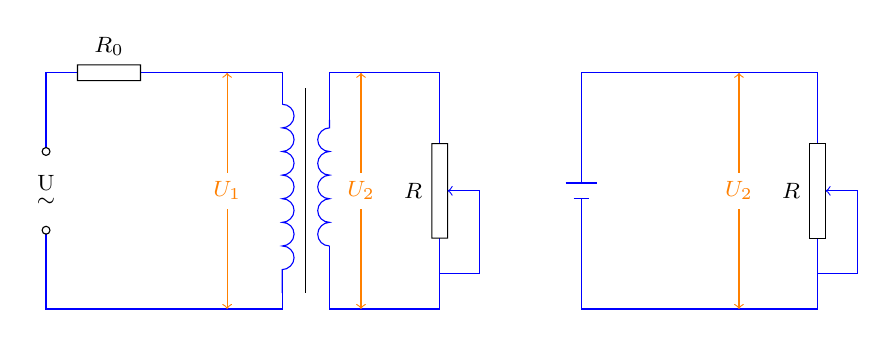
\begin{tikzpicture}[decoration={bumps,segment length=6mm,amplitude=1.5mm}]
			\draw[blue] (0,2)--(0,3)--(3,3)--(3,2.6) (0,1)--(0,0)--(3,0)--(3,.4);
			\draw[decorate,blue] (3,2.6)--(3,.2);
			\draw[blue,decorate] (3.6,.8)--(3.6,2.4);
			\draw[blue] (3.6,2.4)--(3.6,3)--(5,3)--(5,0)--(3.6,0)--(3.6,.8);
			\draw (3.3,2.8)--(3.3,.2);
			\filldraw[fill=white] (0,1) circle(.05) (0,2) circle(.05) (.4,2.9) rectangle(1.2,3.1) (4.9,.9) rectangle(5.1,2.1);
			\draw[blue,->] (5,.45)--(5.5,.45)--(5.5,1.5)--(5.1,1.5);
			\draw[orange,<->] (2.3,0)--node[fill=white]{\footnotesize \(U_1\)}(2.3,3);
			\draw[orange,<->] (4,0)--node[fill=white]{\footnotesize \(U_2\)}(4,3);
			\node at(0,1.6){\footnotesize \(\mathrm{U}\)};
			\node at(0,1.35){\footnotesize \(\sim\)};
			\node at(.8,3.1)[above]{\footnotesize\(R_0\)};
			\node at(4.9,1.5)[left]{\footnotesize\(R\)};
		\begin{scope}[xshift=6.8cm]
			\draw[blue] (0,1.6)--(0,3)--(3,3)--(3,0)--(0,0)--(0,1.4);
			\draw[thick,blue] (-.2,1.6)--(.2,1.6);
			\draw[blue] (-.1,1.4)--(.1,1.4);
			\filldraw[fill=white] (2.9,.9) rectangle(3.1,2.1);
			\draw[blue,->] (3,.45)--(3.5,.45)--(3.5,1.5)--(3.1,1.5);
			\draw[orange,<->] (2,0)--node[fill=white]{\footnotesize \(U_2\)}(2,3);
			\node at(2.9,1.5)[left]{\footnotesize\(R\)};
		\end{scope}
	\end{tikzpicture}
	\end{figure}

	\[
		\begin{aligned}
			U&= U_1 + I_1R_0\\
			U&= \frac{n_1}{n_2}U_2 + \frac{n_2}{n_1}I_2R_0\\
			U_2&= \frac{n_2}{n_1}U -(\frac{n_2}{n_1})^2I_2R_0\\
			&= E - I_2r\\
			E& = \frac{n_2}{n_1}U\qquad r =(\frac{n_2}{n_1})^2R_0\\
		\end{aligned}
	\]